\chapter{Literature Review}
\label{ch:lit_rev} %Label of the chapter lit rev. The key ``ch:lit_rev'' can be used with command \ref{ch:lit_rev} to refer this Chapter.

Bitcoin, a decentralized digital currency, has become more well-known as a substitute for stock market investing. Numerous dangers and factors have the potential to impact the stock market. However, bitcoin is one cryptocurrency that has been steadily increasing in value over the past several years, despite the fact that the value of other cryptocurrencies might suddenly crash without anybody being able to explain why. The stock market requires forecasts about bitcoin from both a human analyst and an automated software because to its volatility. 

Traders are eager to capitalize on the opportunities presented by the thriving Indian stock market at the moment. Because of this, it is important to estimate the Nifty 50's value accurately while trading stocks. The futures and options (F\&O) market component is one of the fundamental indicators of the Nifty 50.Machine learning techniques are used for more precise prediction. The forward neural network, the generalized regression neural network, the radial basis neural network, and the precise radial basis neural network are the four machine-learning-based neural network models we discuss in this study. By comparing the Nifty 50 value with a minimum error rate, four models were offered in the study effort to anticipate the degree of accuracy. In order to finish the research, samples were gathered from the Yahoo Finance website spanning the previous nine years, from January 2013 to June 2021. The original beginning value, day high, day low, and total volumes traded on that day are all considered input characteristics for the Nifty 50 value of the stock market. An output parameter is utilized, which is the day's closing value. The testing results demonstrate that the radial basis neural network model outperforms the other three models with an accuracy of 98.17\%, making it the best model for predicting the Nifty 50 stock market perspectives \citep{lamba2021comparative}.

After being first presented by a group of researchers at Google Brain in 2017, transformers are 
quickly displacing RNN models, such as extended short-term memory, as the preferred model for 
problems with natural language processing (LSTM). White and Safi (2016) demonstrated that when 
the ANN model's linking function was nonlinear, it outperformed the ARIMA model. But the ARIMA 
model did better than the ANN model when its linking function was linear. This is not 
unexpected given that the ARIMA model was created especially for this circumstance 
\citep{safi2021hybrid}. The hybrid model that is employed is a blend of the autoregressive 
integrated moving average (ARIMA) model, the nonlinear artificial neural network (ANN), and the 
Error, Trend, and Seasonality (ETS) models. It is a linear stochastic model. The hybrid model 
outperforms the linear and nonlinear models, according to data from earlier investigations. For 
instance, the hybrid model was shown to have the highest accuracy when used to forecast drought 
in India using a standardized precipitation index series, in comparison to separate stochastic 
and ANN models.

Big data analytics are used to accurately forecast and analyze large data collections. They enable the discovery of valuable information from massive data sets that might otherwise be lost. This research proposes a durable Cloudera-Hadoop-based data pipeline strategy for executing studies for any scale and kind of data, in which chosen US equities are analyzed to estimate daily gains using real-time data from Yahoo Finance. Stocks from the US stock market are chosen, and data on their daily gains is divided into training and test data sets so that Spark's Machine Learning module can forecast the stocks with the highest daily gains. The Apache Hadoop big-data platform is available for handling enormous data collections via distributed storage and processing \citep{peng2019stocks}.
Because of the market's high level of intricacy and volatility, forecasting its behavior is challenging. Researchers are investigating a number of stock market forecasting methodologies to improve accuracy. In this article, we propose using an SBLSTM (Stacked Bidirectional Long Short-Term Memory) network to anticipate stock market movements. To create a deep neural network model, the suggested SBLSTM stacks three bidirectional LSTM networks on top of each other. This method has the potential to increase prediction performance when it comes to stock price forecasts. Unlike LSTM-based approaches, the SBLSTM offered collects temporal data in both forward and backward ways using bidirectional LSTM layers. This method controls the long-term interdependence of the stock market's expected and historical values. The suggested SBLSTM's performance is evaluated using six different Yahoo Finance datasets. Furthermore, the proposed SBLSTM is compared to existing cutting-edge approaches based on root mean square error. According to empirical testing on the dataset \citep{lim2021stacked}, the proposed SBLSTM outperforms state-of-the-art approaches.

Volatility clustering is an important factor that influences how stock markets work. However, developing credible models for accurately anticipating future stock price volatility is a difficult research challenge to address. We provide multiple volatility models based on the generalized autoregressive conditional heteroscedasticity (GARCH) framework for describing the volatility of ten equities listed on India's National Stock Exchange (NSE). The stocks were offered by the Indian economy's banking and car industries, and they have a substantial influence on the sectoral indexes maintained by their respective industries on NSE. Historical stock price data from January 1, 2010, to April 30, 2021 were extracted from the Yahoo Finance website using the Python computer language's Data Reader API. This operation began on January 1, 2010. The training data is used to create and fine-tune the GARCH modules, while the out-of-sample data is used to test the models and evaluate their performance. According to the results, asymmetric GARCH models forecast future stock price volatility more precisely \citep{sen2021volatility}.

Bitcoin is a kind of digital money that is encrypted and hence extremely difficult to reproduce or counterfeit. Blockchain technology serves as the primary foundation for classifying several cryptocurrency networks. The current socioeconomic situation allows consumers to save less cash and remain disconnected from market movements. The project's purpose is to build an effective machine learning prediction model. We begin by downloading data from the Yahoo Finance website using built-in Python modules. Our objective was to apply machine learning to forecast the values of several cryptocurrencies, thus we used the Autoregressive Integrated Moving Average Model (ARIMA). We used lagged data from the previous day, seven days, and thirty days to do feature engineering. We used Plot graph to predict the model's outcome and plot it in a responsive chart \citep{aanandhi2021cryptocurrency}.

In recent years, a rising number of research projects have been launched to investigate the predictability of financial market patterns using a range of machine learning techniques. In this article, we will investigate the possibility of using deep neural networks to assess and anticipate futures market trends. Our technique forecasts futures market movement using enhanced market transaction data and the ARIMA-ANN model. First, we will obtain the ARIMA residual and utilize it to train the ANN model. We train and test our model on a regular basis to check and verify the accuracy of its forecasts. Then, to put our plan to the test, we build and launch a comprehensive trading platform. Our model generates favorable results in both historical back testing and real-time paper trading on this platform. Genuine paper trading yields a total return of 58.69\% over a 12-month period while accounting for slippage and expenses, indicating the efficiency of the strategy outlined \citep{sun2019predicting}.

The usage of social networking sites has become so widespread that they have become an integral part of our everyday life. Users can use this technology to post and view material to their accounts, such as text messages, photos, and videos. Users can engage with one another within their current locations in the same manner that social networking websites do, and publish newly updated information that will be shared with any other followers or guest users. As part of this research effort, we propose a unique way for assessing existing resources in order to predict both sentiment analysis and user expectations. These findings apply to Applied Economics, Expert Systems, Human Brain Analysis, Voting, Stock Markets, Live Updates on Any Field, and other areas \citep{ramesh2020artificial}.

Machine learning algorithms enable computers to discover patterns in data sets and generate predictions using statistical approaches, which is only one component of the process. During the machine learning process, a grouping model is created from the data set to predict the kind of test data based on the training data. Every sector is currently looking into machine learning in order to produce solutions that are dependable, precise, and optimized. This is evident in the financial industry, e-commerce, stock markets, healthcare, the automation of daily human work, and wildlife protection. Machine learning techniques include linear regression, logistic regression, decision trees, random forests, K-means clustering, artificial neural networks, and deep learning architectures. Because of their distinct qualities, these methods may be utilized as either classification or regression models \citep{ponnam2016comparative}.

To make lucrative investments, businesspeople and the middle class need be informed of stock market forecasts. This article makes use of the company's dynamic dataset. The dataset contains the stock's value at the end of each of the last 290 working days. The dataset was acquired from Yahoo Finance (https://finance.yahoo.com), thus the information in it is reliable. To accurately anticipate the stock market, an acceptable approach for the dataset was selected. A number of technical analysis and machine learning approaches are used to forecast the company's stock and exchange rate values in the future. This article uses a variety of machine learning models, including Linear Regression, Decision Tree, Random Forest, SVR, ANN, LSTM, Lasso Regression, KNN, Bayesian Ridge, ARIMA, Gradient Boosting, and Ada Boost \citep{yasmin2022stock}.

\chapter{Time Series}

A time series is a set of data points that appear in a specific order over a given period of time. This is comparable to cross-sectional data, which represents a single moment in time. An investment time series collects data points at regular intervals and plots the change of those data points, such as the price of an asset, over time. Because there is no minimum or maximum amount of time that must be included, the data may be collected in such a way that the investor or analyst looking at the activity receives the information they want.

\section{Understanding Time Series} %  use this section 
\label{sec:intro_sum_results} % label of summary of results
A time series may be used to represent any variable that varies over time. A time series is commonly used in investing to track the price of an investment over time. This can be done over a short period of time, such as a security's price at each hour throughout a business day, or over a long period of time, such as the price of a security at the end of each month during a five-year period.
Time series analysis may be useful in determining how a certain asset, security, or economic variable evolves over time. It may also be used to compare changes in the selected data point to changes in other variables within the same time period.

\begin{figure}[ht]
    \centering
    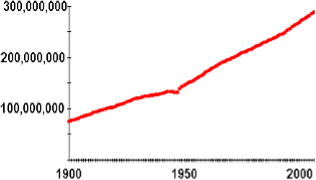
\includegraphics[scale=1.0]{figures/TimeSeries.png}
    \caption{A time series graph of the population of the United States from 1900 to 2000.}
    \label{fig:chart_a}
\end{figure}

\section{Time Series Analysis} %  use this section 
\label{sec:intro_sum_results} % label of summary of results
For a given stock, you may look at a whole year's worth of daily closing prices. You would generate a list of the stock's closing prices for the previous year, in reverse chronological order. This would be an annual time series of the stock's daily closing prices.

whether you want to dig deeper, you might utilize technical analysis tools to evaluate time series data to see whether the stock's time series has any seasonality. This can help you determine whether the stock has peaks and troughs at regular periods throughout the year. For this region's study, the observed prices would need to be compared to a certain season. This can encompass both ordinary calendar seasons, such as summer and winter, and commercial seasons, such as the Christmas shopping season.

Alternatively, a stock's share price history can be traced in connection to economic indicators such as the unemployment rate. Patterns can be identified in situations where the data points and the chosen economic variable are dependant by connecting the data points with knowledge of that variable. Because each variable in a time series is dependent on its prior condition or value, there may be a high number of autocorrelations, skewing the findings.



\section{Time Series Forecasting} %  use this section 
\label{sec:intro_sum_results} % label of summary of results
Time series forecasting uses previous values and trends to anticipate the future of activity. This generally involves trend analysis, cyclical fluctuation analysis, and seasonality issues. Any forecasting approach cannot be guaranteed to succeed.

For example, the Box-Jenkins Model is a technique for forecasting data ranges using inputs from a certain time series. Data forecasting employs three concepts: autoregression, differencing, and moving averages. These three principles are named P, D, and Q. Each principle is used in the Box-Jenkins analysis, and when combined, they produce an ARIMA (p, d, q). ARIMA, for example, can be used to forecast stock price movements or revenue growth.

Rescaled range analysis is an alternative approach for identifying and quantifying persistence, unpredictability, and mean reversion in time series data. To evaluate if a trend is stable or likely to reverse, use the rescaled range to estimate a future value or average.

\section{Cross-Sectional vs. Time Series Analysis} %  use this section 
\label{sec:intro_sum_results} % label of summary of results
Cross-sectional analysis is one of two primary stock comparison methodologies. Cross-sectional analysis is used to assess data obtained at a particular moment in time rather than throughout time. The initial steps in the analysis process are to define the variables an analyst wants to assess and set research objectives. The next step is to select the cross section to be examined, such as a group of peers or an industry, as well as the specific time period. The next stage is to conduct analysis based on the variables and cross section, and then make a judgment on how well a business or organization is operating. Cross-sectional analysis selects the best business for an investor based on the factors that are important to them.

When employed in technical trading, time series analysis, also known as trend analysis, focuses on a single securities across time. In this case, the price is determined by its historical performance. An investor can use time series analysis to identify whether a firm is performing better or worse than it was previously depending on the parameters that are important to them. These are often classic indicators like as profits per share (EPS), debt to equity, free cash flow (FCF), and so on. When making a decision, investors commonly mix time series with cross-sectional analysis—for example, by first studying EPS over time and then comparing it to industry benchmark EPS.
